\documentclass{article}
\usepackage{pythonhighlight}
\usepackage{graphicx}
\usepackage{ctex}
\usepackage[left=3cm,top=3cm,right=3cm]{geometry}
\usepackage{hyperref}
% TITLE PAGE CONTENT %%%%%%%%%%%%%%%%%%%%%%%%
%%%%%%%%%%%%%%%%%%%%%%%%%%%%%%%%%%%%%%%%%%%%%
\newcommand{\labno}{10}
\newcommand{\labtitle}{EE208 Histogram}
\newcommand{\authorname}{周李韬}
\newcommand{\studentno}{518030910407}
\newcommand{\classno}{F1803016}
% END TITLE PAGE CONTENT %%%%%%%%%%%%%%%%%%%%


\begin{document}

\begin{center}
{\LARGE \textsc{Laboratory No. \labno:} \\ \vspace{4pt}}
{\Large \textsc{\labtitle} \\ \vspace{4pt}} 
\rule[13pt]{\textwidth}{1pt} \\ \vspace{15pt}
{\large By: \authorname \\ \vspace{10pt}
No. \studentno \\ \vspace{10pt}
SJTU \classno \\ \vspace{10pt}
\today \vspace{20pt}}
\end{center}



\section{实验准备}

\subsection{实验环境}
\begin{itemize}
\item\textbf{Environment} Python 3.7
\item\textbf{Packages} numpy 1.15.4, opencv-python 3.4.3.18
\item\textbf{Tools} Pycharm 2018.2 on Windows 10
\end{itemize}

\subsection{实验目的}

本实验中,我们需要练习使用opencv读取图片,并计算图片的颜色直方图、灰度直方图和灰度梯度直方图。

\subsection{实验原理}

像素是图像的基本元素,一幅图像在计算机中用一个长$\times$宽的矩阵存储。灰度图像中每一个对应像素的灰度值范围在0-255之间,彩色图像则由红、绿、蓝三个通道组成。本实验中,我们可以通过遍历图像的像素矩阵,统计或计算颜色直方图、灰度直方图和梯度直方图所需要的数据。


\section{实验步骤}

\subsection{颜色直方图}
颜色直方图的计算需要统计三个颜色总能量的相对比例。我们可以统计某一颜色分量的总能量:
\begin{equation}
E(c)=\sum_{x=0}^{W-1} \sum_{y=0}^{H-1} I(x, y, c)
\end{equation}
从而计算某一颜色分量的能量相对比例。
\begin{equation}
H(c)=\frac{E(c)}{\sum_{i=0}^{2} E(i)}
\end{equation}

统计颜色直方图的Python脚本如下,openCV中,颜色的三个通道作为每一个像素对应矩阵元素的三个分量体现。
\begin{python}
img = cv2.imread(image_dir, cv2.IMREAD_COLOR) # 以彩色格式读入图像
EB = 0
EG = 0
ER = 0
for rows in img:        # 遍历像素
    for i in rows:      # 统计每一个颜色分量的能量值
        EB += i[0]
        EG += i[1]
        ER += i[2]
E = EB + EG + ER        # 计算总能量
\end{python}

\subsection{灰度直方图}
灰度图像$I(x,y)$的灰度直方图定义为各灰度值像素数目的相对比例。
图像中灰度值为i的像素总个数为:
\begin{equation}
N(i)=\sum_{x=0}^{W-1} \sum_{y=0}^{H-1} I(x, y)=i ? 1: 0
\end{equation}
灰度直方图第i项分量的值为
\begin{equation}
H(i)=\frac{N(i)}{\sum_{j=0}^{255} N(j)}, i=0, \cdots 255
\end{equation}

我们在Python中用类似的思想遍历像素矩阵,将每一个灰度值的统计数记录在一个长度为256的列表中,即可得到绘制灰度直方图所需的数据。
\begin{python}
N_table = [0] * 256
for rows in img:            # 遍历像素矩阵,统计灰度值个数
    for i in rows:
        N_table[i] += 1
for i in range(256):        # 计算灰度值对应像素所占比例并输出
    f.write(str(N_table[i]/size) +'\n')
\end{python}



\subsection{梯度直方图}
假设$I(x, y)$表示一幅灰度图像,则它$X$方向的梯度定义为:
\begin{equation}
I_{x}(x, y)=\frac{\partial I(x, y)}{\partial x}=I(x+1, y)-I(x-1, y)
\end{equation}
$Y$方向的梯度定义为:
\begin{equation}
I_{y}(x, y)=\frac{\partial I(x, y)}{\partial y}=I(x, y+1)-I(x, y-1)
\end{equation}
梯度强度定义为
\begin{equation}
M(x, y)=\sqrt{I_{x}(x, y)^{2}+I_{y}(x, y)^{2}}
\end{equation}

本实验中忽略了边界像素的梯度,因此计算的范围是1~Width-2,1~Height-2的像素点梯度。在Python脚本中,我们先计算当前点的梯度,随后取整,根据计算结果统计到一个长度为361(梯度的最大值)的列表中,作为绘制直方图的依据。
\begin{python}
M_table = [0]*361
for i in range(1,height-1):
    for j in range(1,width-1):
        b_i = int(img[i+1][j])-int(img[i-1][j])
        b_j = int(img[i][j+1])-int(img[i][j-1])
        m = int(math.sqrt(b_i*b_i+b_j*b_j))    # 计算灰度梯度值,取整
        M_table[m] += 1                        # 统计

grad_size = (width-2)*(height-2)
for idx in range(361):
    f.write(str(M_table[idx]/ grad_size)+'\n') # 输出灰度梯度比例
\end{python}

\subsection{输入输出}
为方便数据的收集,我们将每一类直方图的计算封装成一个函数,函数的输入接口是图片文件和输出文件地址,执行完函数后,结果会被输出到一个文本文件中。Python脚本中的函数结构和调用方式示例如下。

\begin{python}
def get_color_histogram(output_file,image_dir):
    ...
    
if __name__ == '__main__':
    get_color_histogram("./result/1_1.txt","./images/img1.png")
    ...
\end{python}


\section{实验结果}

我们用Excel对实验结果绘制直方图,绘制结果如下。源数据及图表可以在附加材料的xls工作簿中找到。

\begin{figure}[htb]
\centering
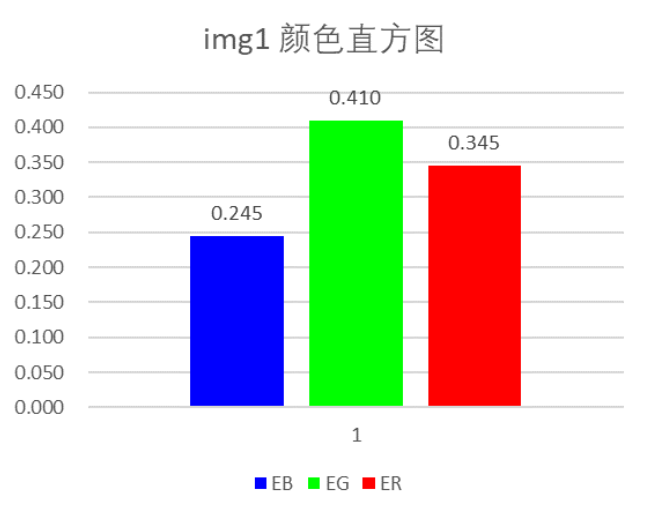
\includegraphics[width=7.5cm]{img/1-1.png}
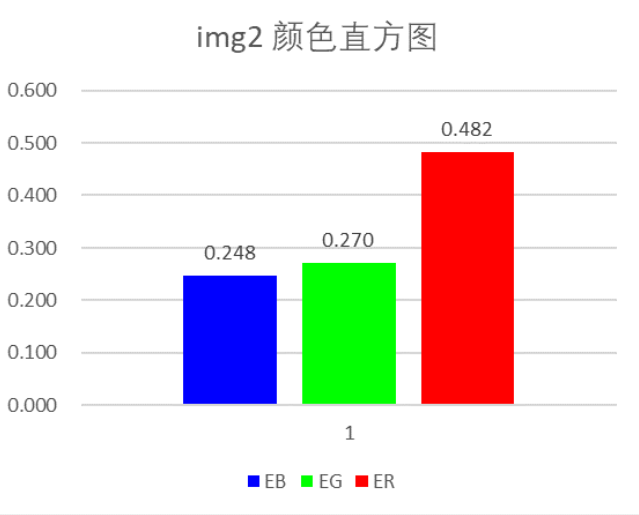
\includegraphics[width=7.5cm]{img/1-2.png}
\caption{颜色直方图}
\label{1}
\end{figure}

\begin{figure}[htb]
\centering
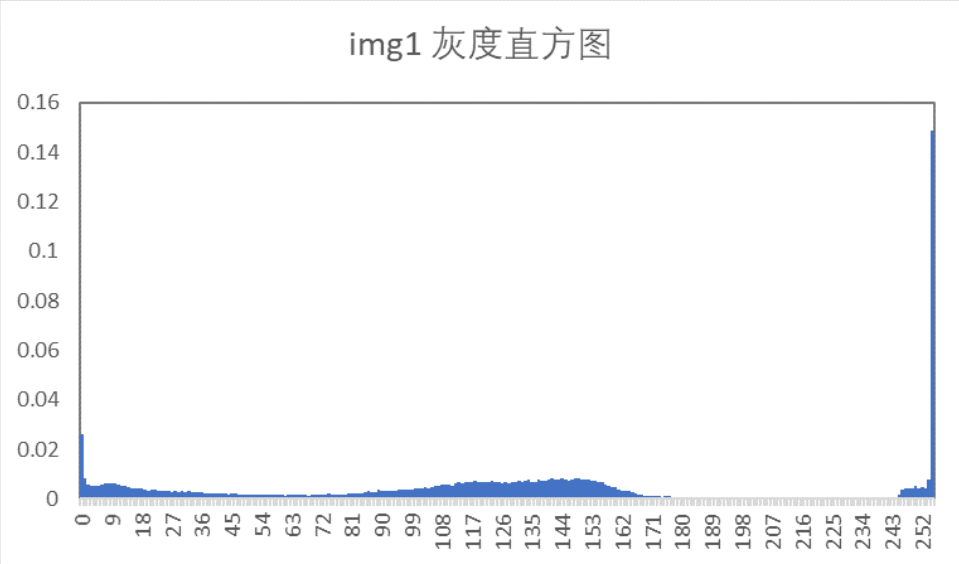
\includegraphics[width=13.5cm]{img/2-1.png}
\caption{灰度直方图}
\label{2}
\end{figure}
\begin{figure}[htb]
\centering
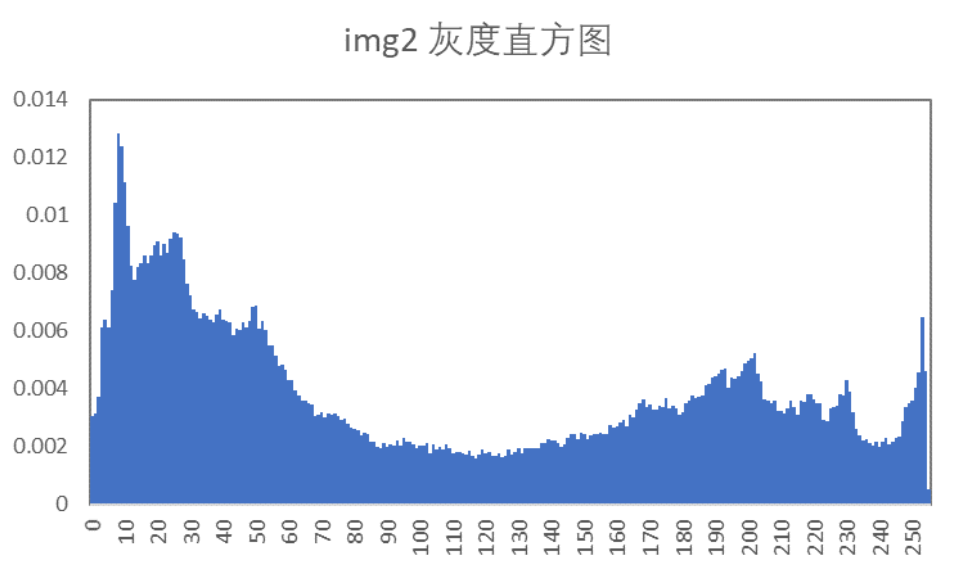
\includegraphics[width=13.5cm]{img/2-2.png}
\caption{灰度直方图}
\label{2.2}
\end{figure}

\begin{figure}[htb]
\centering
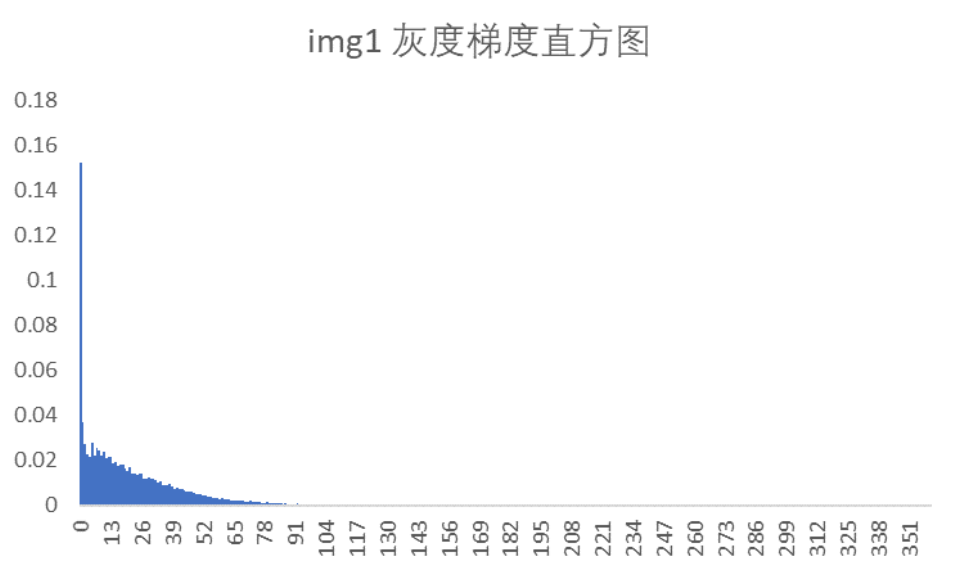
\includegraphics[width=13.5cm]{img/3-1.png}
\caption{灰度梯度直方图}
\label{3}
\end{figure}

\begin{figure}[htb]
\centering
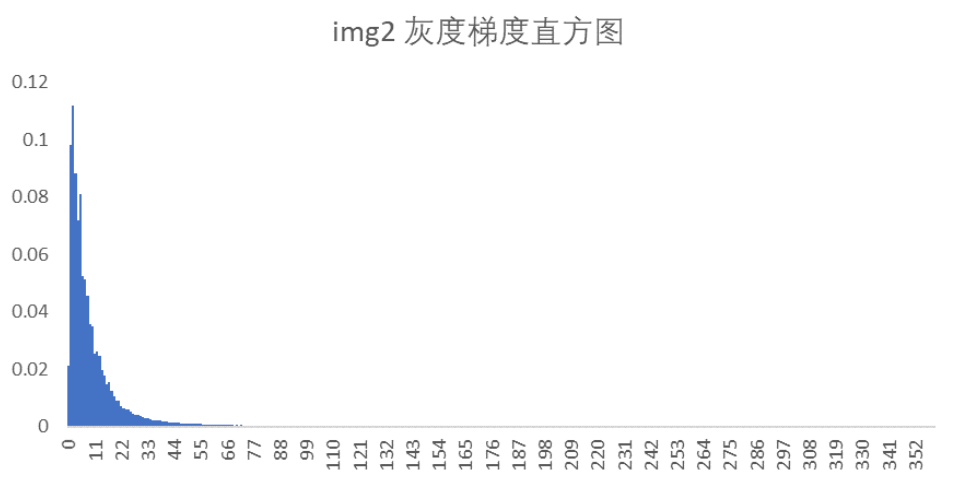
\includegraphics[width=13.5cm]{img/3-2.png}
\caption{灰度梯度直方图}
\label{3.2}
\end{figure}

\section{实验总结}
\paragraph{概述}
本实验中,我们通过OpenCV读取了两张图片中的像素数据,并绘制了其对应的颜色直方图、灰度直方图和梯度直方图。

\paragraph{感想}
通过本次实验的学习,我加强了图片像素构成的认识,学会了使用OpenCV对像素进行操作的技巧,同时也对图像处理中的梯度概念有了更深的理解。

\paragraph{创新}
本实验中对获取图片直方图数据的Python脚本做了封装,能够实现数据的外部存储,增强了可用性。

\end{document}

